\documentclass[a4paper,11pt,titlepage]{scrbook}
\usepackage[utf8]{inputenc} %codificacion
\usepackage[spanish]{babel} %idioma

%\usepackage{titlesec}
%\usepackage{palatino} %usar fot palatino en vez de times roman

%\decimalpoint %revisar
%\usepackage{dcolumn} %revisat
%\newcolumntype{.}{D{.}{\esperiod}{-1}}
%\makeatletter
%\addto\shorthandsspanish{\let\esperiod\es@period@code}
%\makeatother


%\usepackage[chapter]{algorithm}
%\RequirePackage{verbatim}
%\RequirePackage[Glenn]{fncychap}
\usepackage{fancyhdr} %estilo del documento
\usepackage{graphicx} %colores
\usepackage{afterpage} %\clearpage y un par mas de funcs
\usepackage{longtable} %tabular and table extra opcs
\usepackage{xcolor}   %opcs colores
\definecolor{portada}{RGB}{239,206,53}
\definecolor{base}{RGB}{35,31,32}
\usepackage{pdfpages} %inclusion de archivos al doc
\usepackage[acronym]{glossaries} %acronimos y abreviaturas
\usepackage{acronym}
\usepackage{breakcites} %modifica \cite
\usepackage{natbib}

\renewcommand{\glossaryname}{Glosario}
\renewcommand{\acronymname}{Acrónimos}

%Instrucciones para poder escribir código y mostrarlo de manera elegante:
\definecolor{gray97}{gray}{.97}
\definecolor{gray75}{gray}{.75}
\definecolor{gray45}{gray}{.45}
\definecolor{gray30}{gray}{.94}

\usepackage{listings} %para escribir codigo
\lstset{ frame=Ltb,
framerule=0pt,
aboveskip=0.5cm,
framextopmargin=3pt,
framexbottommargin=3pt,
framexleftmargin=0.4cm,
framesep=0pt,
rulesep=.4pt,
backgroundcolor=\color{gray97},
rulesepcolor=\color{black},
%
stringstyle=\ttfamily,
showstringspaces = false,
basicstyle=\small\ttfamily,
commentstyle=\color{gray45},
keywordstyle=\bfseries,
%
numbers=left,
numbersep=15pt,
numberstyle=\tiny,
numberfirstline = false,
breaklines=true,
literate={á}{{\'a}}1 {Á}{{\'A}}1 {é}{{\'e}}1 {É}{{\'e}}1 {í}{{\'i}}1  {Í}{{\'I}}1  {ó}{{\'o}}1  {Ó}{{\'O}}1  {ú}{{\'u}}1  {Ú}{{\'U}}1  {Ñ}{{\~N}}1 {ñ}{{\~n}}1 ,
}



% minimizar fragmentado de listados
\lstnewenvironment{listing}[1][]
   {\lstset{#1}\pagebreak[0]}{\pagebreak[0]}

\lstdefinestyle{Consola}
   {basicstyle=\scriptsize\bf\ttfamily,
    backgroundcolor=\color{gray30},
    frame=single,
    numbers=none
   }
\lstdefinestyle{C}
	{basicstyle=\scriptsize,
	frame=single,
	language=C,
	numbers=left
	}
\lstdefinestyle{CodigoC++}
        {basicstyle=\small,
	frame=single,
	backgroundcolor=\color{gray30},
	language=C++,
	numbers=left
 	}
\lstdefinestyle{PHP}
	{basicstyle=\scriptsize,
%        {basicstyle=\small,
	frame=single,
	language=PHP,
	numbers=left
	}
	
%OPCS PROPIAS
\setlength{\parskip}{.8em}
%


% ********************************************************************
% Información sobre el TFG. Comentar lo que NO se desee añadir y sustituir con la información correcta.
% ********************************************************************
\newcommand{\myTitle}{Título del Trabajo de Fin de Grado}
\newcommand{\mySubtitle}{Gestión y manejo de comportamientos grupales 
\\ de entidades en videojuegos}
\newcommand{\myDegree}{Grado en Ingeniería Multimedia}
\newcommand{\myName}{Borja Pozo Wals}
\newcommand{\myProf}{Francisco José Gallego Durán}
%\newcommand{\myOtherProf}{Nombre Apellido1 Apellido2 (tutor2)}
\newcommand{\myFaculty}{Escuela Politécnica Superior de la Universidad de Alicante}
\newcommand{\myFacultyShort}{EPS UA}
\newcommand{\depTutorOne}{Departamento de Ciencia de la Computación e Inteligencia Artificial}
%\newcommand{\depTutorTwo}{Departamento del cotutor}


\newcommand{\myUni}{\protect{Universidad de Alicante}}
\newcommand{\myLocation}{Alicante}
\newcommand{\myTime}{\today}
%\newcommand{\myVersion}{Version 0.1}

\newcommand{\logoGrado}{imagenes/logoim.jpg}
\newcommand{\logoFacultad}{imagenes/logoeps.jpg}
\newcommand{\logoUniversidad}{imagenes/logoua.jpg}

\usepackage{url}

% Definición de comandos que me son útiles:
%\renewcommand{\indexname}{Índice alfabético}
%\renewcommand{\glossaryname}{Glosario}

\pagestyle{fancy}
\fancyhf{}
\fancyhead[LO]{\leftmark}
\fancyhead[RE]{\rightmark}
\fancyhead[RO,LE]{\textbf{\thepage}}
\renewcommand{\chaptermark}[1]{\markboth{\textbf{#1}}{}}
\renewcommand{\sectionmark}[1]{\markright{\textbf{\thesection. #1}}}


\setlength{\headheight}{1.5\headheight}

\newcommand{\HRule}{\rule{\linewidth}{0.5mm}}
%Definimos los tipos teorema, ejemplo y definición podremos usar estos tipos
%simplemente poniendo \begin{teorema} \end{teorema} ...
\newtheorem{teorema}{Teorema}[chapter]
\newtheorem{ejemplo}{Ejemplo}[chapter]
\newtheorem{definicion}{Definición}[chapter]
 
\newcommand{\bigrule}{\titlerule[0.5mm]}


%Para conseguir que en las páginas en blanco no ponga cabeceras
\makeatletter
\def\clearpage{%
  \ifvmode
    \ifnum \@dbltopnum =\m@ne
      \ifdim \pagetotal <\topskip
        \hbox{}
      \fi
    \fi
  \fi
  \newpage
  \thispagestyle{empty}
  \write\m@ne{}
  \vbox{}
  \penalty -\@Mi
}
\makeatother

\usepackage[pdfborder={000}]{hyperref} %referencia
\hypersetup{
pdfauthor = {\myName (bpw1@alu.ua.es)},
pdftitle = {\myTitle},
pdfsubject = {},
pdfkeywords = {AI, Inteligencia Artificial, Videojuegos, C++},
pdfcreator = {LaTeX con el paquete ....},
pdfproducer = {pdflatex}
}
%AQUI COMIENZA LA LISTA DE FICHEROS A INCLUIR


\begin{document}
\renewcommand{\listtablename}{Índice de tablas} %para sustituir la palabra cuadro por tabla
\renewcommand{\tablename}{Tabla}
\renewcommand{\lstlistingname}{Listado}
\renewcommand{\lstlistlistingname}{Índice de \lstlistingname s}

\frontmatter
\begin{titlepage}

\newlength{\centeroffset}
\setlength{\centeroffset}{-0.5\oddsidemargin}
\addtolength{\centeroffset}{0.5\evensidemargin}
\thispagestyle{empty}

\includepdf[pages={1},pagecommand={},fitpaper=true,trim=0 0 0 0, 
offset=0 0,turn=true,noautoscale=true]{portada/portada.pdf}

\end{titlepage}
\pagecolor{white} %la portada en color
\begin{titlepage}
 
 
\setlength{\centeroffset}{-0.5\oddsidemargin}
\addtolength{\centeroffset}{0.5\evensidemargin}
\thispagestyle{empty}

\noindent\hspace*{\centeroffset}\begin{minipage}{\textwidth}

\centering


% Title

%{\Huge\bfseries Título del proyecto\\ }
{\Huge\bfseries \myTitle}

\noindent\rule[-1ex]{\textwidth}{3pt}\\[3.5ex]
{\large\bfseries \mySubtitle\\[4cm]}
\end{minipage}

\vspace{2.5cm}
\noindent\hspace*{\centeroffset}\begin{minipage}{\textwidth}
\centering

\textbf{Autor}\\ {\myName}\\[2.5ex]
\textbf{Tutor/es}\\
{\normalsize \myProf\\
\small\textit \depTutorOne\\[6cm]}
%\normalsize \myOtherProf\\
%\small\textit \depTutorTwo

\includegraphics[scale=0.75]{\logoGrado}


\textsc{\myDegree}\\[4mm]

\centering
\begin{minipage}[l]{7cm}
\includegraphics[width=5cm]{\logoFacultad}
\end{minipage}
\begin{minipage}[r]{7cm}
\hspace{1cm}
\includegraphics[width=5cm]{\logoUniversidad}
\end{minipage}\\[0.4cm]


%\textsc{\myFaculty}\\

%\large\bfseries \textsc{\myUni}\\
ALICANTE, \myTime

\end{minipage}
%\addtolength{\textwidth}{\centeroffset}
\vspace{\stretch{2}}

\end{titlepage}


 %la portada en b/n
%\chapter*{Preámbulo}
\thispagestyle{empty}
\textbf{titulo por definir} es una herramienta para simular escenarios 
 bélicos como los que podemos encontrar en juegos del género \ac{RTS} como son
 `Mount \& Blade' o la saga `Imperium', desarrollado completamente en C++ para \ac{PC}.

La simulación se compone de un escenario, una unidad controlada por el jugador,
una serie de unidades que conforman el ejercito bajo sus ordenes y por último, 
tenemos una serie de objetivos que abatir. Una vez conseguido el objetivo terminará
el juego pudiendo el jugador elegir entre repetir el nivel o volver al menú principal.


\cleardoublepage %salta a nueva página impar
\chapter*{Agradecimientos\footnote{Por si alguien tiene curiosidad, este ``simpático'' agradecimiento está tomado de la ``Tesis de Lydia Chalmers'' basada en el universo del programa de televisión Buffy, la Cazadora de Vampiros.http://www.buffy-cazavampiros.com/Spiketesis/tesis.inicio.htm}
}

\thispagestyle{empty}
\vspace{1cm}

Este trabajo no habría sido posible sin el apoyo y el estimulo de mi colega y amigo, Doctor Rudolf Fliesning,  bajo cuya supervisión escogí este tema y comencé la tesis. Sr. Quentin Travers, mi consejero en las etapas finales del trabajo, también ha sido generosamente servicial, y me ha ayudado de numerosos modos, incluyendo el resumen del contenido de los documentos que no estaban disponibles para mi examen, y en particular por permitirme leer, en cuanto estuvieron  disponibles, las copias de los  recientes extractos de los diarios de campaña del Vigilante Rupert Giles y la actual Cazadora la señorita Buffy Summers, que se encontraron con William the Bloody en 1998, y por facilitarme el pleno acceso  a los diarios de anteriores Vigilantes relevantes a la carrera de William the Bloody.

También me gustaría agradecerle al Consejo la concesión de Wyndham-Pryce como Compañero, el cual me ha apoyado durante mis dos años de investigación, y la concesión de dos subvenciones de viajes, una para estudiar documentos en los Archivos de Vigilantes sellados en Munich, y otra para la investigación en campaña en Praga. Me gustaría agradecer a Sr. Travers, otra vez, por facilitarme  la acreditación  de seguridad para el trabajo en los Archivos de Munich, y al Doctor Fliesning por su apoyo colegial y ayuda en ambos viajes de investigación.

No puedo terminar sin agradecer a mi familia, en cuyo estímulo constante y amor he confiado a lo largo de mis años en la Academia. Estoy agradecida también a los ejemplos de mis  difuntos hermano, Desmond Chalmers, Vigilante en Entrenamiento, y padre, Albert Chalmers, Vigilante. Su coraje resuelto y convicción siempre me inspirarán, y espero seguir, a mi propio y pequeño modo, la noble misión por la que dieron sus vidas. 

Es a ellos a quien dedico este trabajo.

\cleardoublepage %salta a nueva página impar
% Aquí va la dedicatoria si la hubiese. Si no, comentar la(s) linea(s) siguientes
\chapter*{}
\setlength{\leftmargin}{0.5\textwidth}
\setlength{\parsep}{0cm}
\addtolength{\topsep}{0.5cm}
\begin{flushright}
\small\em{
A mi esposa Marganit, y a mis hijos Ella Rose y Daniel Adams,\\
sin los cuales habría podido acabar este libro dos años antes \footnote{Dedicatoria de Joseph J. Roman en "An Introduction to Algebraic Topology"}
}
\end{flushright}


\cleardoublepage %salta a nueva página impar
% Aquí va la cita célebre si la hubiese. Si no, comentar la(s) linea(s) siguientes
\chapter*{}
\setlength{\leftmargin}{0.5\textwidth}
\setlength{\parsep}{0cm}
\addtolength{\topsep}{0.5cm}
\begin{flushright}
\small\em{
Si consigo ver más lejos\\
es porque he conseguido auparme\\ 
a hombros de gigantes
}
\end{flushright}
\begin{flushright}
\small{
Isaac Newton.
}
\end{flushright}
\cleardoublepage %salta a nueva página impar

\chapter*{Resumen}
\label{Resumen}
%\thispagestyle{empty}
\textbf{titulo por definir} es una herramienta para simular escenarios 
 bélicos como los que podemos encontrar en juegos del género \ac{RTS} como son
 `Mount \& Blade' o la saga `Imperium', desarrollado completamente en C++ para \ac{PC}.

La simulación se compone de un escenario, una unidad controlada por el jugador,
una serie de unidades que conforman el ejercito bajo sus ordenes y por último, 
tenemos una serie de objetivos que abatir. Una vez conseguido el objetivo terminará
el juego pudiendo el jugador elegir entre repetir el nivel o volver al menú principal.

\chapter*{Justificación y objetivos}
A lo largo de la carrera son muchas las asignaturas que requieren y desarrollan
habilidades relacionadas con la programación en diversos lenguajes y usos, 
pero no es hasta el tercer año que se me presenta la oportunidad de desarrollar
un videojuego completo. 

Durante la asignatura de `Fundamentos de los Videojuegos' tuve por primera vez
la experiencia de enfrentarme al desafio que es crear un videojuego, y fue en ese
momento cuando me di cuenta de que a lo que me quería dedicar es a
desarrollar juegos de forma profesional. A lo largo del cuarto curso junto a los demás
integrantes de \textit{'Sunlight Studio'} desarrollamos \textit{'Cyborgeddon'}, y fue
en este momento que terminé de decidir que es a lo quiero dedicarme en el futuro.

A lo largo de mi vida he jugando una considerable cantidad de juegos entre los cuales
se puede apreciar una inclinación por los juegos de aventura y exploración, los 
\ac{RPG} y los \ac{RTS} o de estrategia en general, es por esto que me hace especial
ilusión desarrollar un juego de uno de estos géneros.\\
Teniendo en cuenta esto la elección de desarrollar un juego del tipo \ac{RTS} para la
realización del \ac{TFG} se debe a que según mi criterio es el que tiene mayor
potencial para ayudarme a mejorar mis habilidades como programador, ya que se basa en
unas mecánicas con las que no he trabajado con anterioridad.

Una vez dicho esto, los objetivos planteados para el proyecto son los siguientes:
\begin{itemize}
	\item Aumentar mis conocimientos de C++
	\item Comprender mejor el funcionamiento del \ac{PC}
	\item Aprender nuevas técnicas de \ac{IA}
	\item Desarrollar un producto mediante el cual mostrar mis habilidades
\end{itemize}

\cleardoublepage %salta a nueva página impar
% Aquí va la dedicatoria si la hubiese. Si no, comentar la(s) linea(s) siguientes
\chapter*{Agradecimientos}
\setlength{\leftmargin}{0.5\textwidth}
\setlength{\parsep}{0cm}
\addtolength{\topsep}{0.5cm}
\begin{flushright}
\small\em{
A mi madre Gabriela,\\
por el increíble esfuerzo que realiza cada día por mi. 
}
\end{flushright}
\begin{flushright}
\small\em{
A mi hermana Raquel,\\
por haber sido y ser un faro para mi. 
}
\end{flushright}
\begin{flushright}
\small\em{
A mi buen compañero Jorge Espinosa,\\
por nuestra convivencia estos años. 
}
\end{flushright}
\begin{flushright}
\small\em{
A mi querido amigo Guillermo y su familia,\\
por el cariño recibido incluso a pesar de la distancia. 
}
\end{flushright}

\cleardoublepage %salta a nueva página impar
% Aquí va la cita célebre si la hubiese. Si no, comentar la(s) linea(s) siguientes
\chapter*{}
\setlength{\leftmargin}{0.5\textwidth}
\setlength{\parsep}{0cm}
\addtolength{\topsep}{0.5cm}
\begin{flushright}
\small\em{
Ni los reyes ni los gobernantes llevan el cetro,\\
sino los que saben mandar\\ 
}
\end{flushright}
\begin{flushright}
\small{
Sócrates.
}
\end{flushright}

\begin{flushright}
\small\em{
Para saber hablar es preciso saber escuchar\\
}
\end{flushright}
\begin{flushright}
\small{
Plutarco.
}
\end{flushright}
\cleardoublepage %salta a nueva página impar
 %editar este texto (capitulos/preliminares.tex) para cambiar preámbulo, agradecimientos y dedicatorias
\tableofcontents
\listoffigures
\listoftables
\lstlistoflistings
\chapter*{Índice de Acrónimos}
\label{acronimos}
% fichero para poner los acrónimos
%para escribir un acrónimo nuevo, seguir el siguiente protocolo: (POR EJEMPLO PARA PONER EL ACRÓNIMO IEEE)
%- En el texto, poned \ac{IEEE}
%- En el fichero acrónimos.tex, poner la siguiente enTrada:
% \acrodef{IEEE}{Institute of Electrical and Electronics Engineers}
% IEEE: Institute of Electrical and Electronics Engineers

%Además de \ac{IEEE} se pueden usar otras fórmulas en el texto para variar el comportamiento del paquete de acrónimos:
% Por ejemplo:
% acf{} hace que siempre aparezca el texto completo del acrónimo correspondiente. (fórmula larga y corta)
% acl{} hace que Solo aparezca la fórmula larga
% acs{} hace que aparezca obligatoriamente la fórmula corta
% acp{} incluye el plural del acrónimo.
% acs{} hace que aparezca la versión córta del acrónimo.
% acresetall{} resetea todos los acrónimos de forma que se establecen como “no usados”.
% acused{} marca el acrónimo como “usado”.

A lo largo del documento serán utilizadas una serie de abreviaturas con el fin de
hacer más cómoda su lectura. Todos los términos están indicados a continuación: 

\begin{itemize}

\acrodef{TFG}{Trabajo Final de Grado}
\acrodefplural{TFG}[TFG]{Trabajos Finales de Grado}
\item \textbf{TFG:} Trabajo Final de Grado

\acrodef{PC}{Personal Computer}
\acrodefplural{PC}[PC]{Personal Computers}
\item \textbf{PC:} Personal Computer

\acrodef{RTS}{Real Time Strategy}
\item \textbf{RTS:} Real Time Strategy

\acrodef{RPG}{Rol Play Game}
\acrodefplural{RPG}[RPG]{Rol Play Games}
\item \textbf{RPG:} Rol Play Game

\acrodef{IA}{Inteligencia Artificial}
\acrodefplural{IA}[IA]{Inteligencias Artificiales}
\item \textbf{IA:} Inteligencia Artificial

\acrodef{NPC}{Non-Player Character}
\acrodefplural{NPC}[NPC]{Non-Player Characters}
\item \textbf{NPC:} Non-Player Character

\acrodef{AoE}{Age of Empires}
\acrodefplural{AoE}[AoE]{Age of Empires}
\item \textbf{AoE:} Age of Empires

\acrodef{TaB}{They are Billions}
\acrodefplural{TaB}[TaB]{They are Billions}
\item \textbf{TaB:} They are Billions

%borrar
\acrodef{TFM}{Trabajo Final de Master}
\acrodef{IEEE}{Institute of Electrical and Electronics Engineers}
\acrodef{EPS}{Escuela Politécnica Superior} 
\acrodef{APA}{American Psychological Association}

\end{itemize}

\mainmatter %entre frontmatter y mainmatter, la numeración es en romanos.

%a continuación se propone un esquema de trabajo que puede ser alterado justificadamente.
\acresetall{}  % resetea los acrónimos por si han sido usados en el índice o en los preliminares.
\chapter{Introducción}
\label{intro}
Este proyecto trata sobre el desarrollo de un simulador de batallas para \ac{PC}
desarrollado en \textit{Linux}, escrito en C++ y haciendo uso de librerias escritas en
C como TinyPTC *add reference*.

El simulador, \textbf{inserte título}, se trata de una demo del género \ac{RTS}
compuesta por un escenario a través del cual tendremos que comandar y luchar junto a
nuestro ejercito con el fin de abatir al ejercito rival. El escenario estará compuesto
por estructuras y obstáculos que deberemos sortear para alcanzar nuestro objetivo.

A nivel técnico el proyecto cuenta con el desafio de desarrollar una \ac{IA} grupal
para los \ac{NPC} basada en el uso de técnicas como los \textit{Steering behaviours} 
y el \textit{Flocking} con el fin de emular un comportamiento coordinado entre las
distintas entidades. El objetivo es crear una versión inicial sencilla mediante la 
cual poder profundizar en los conceptos en los cuales se basan las mencionadas técnicas
con el fin de desarrollar una versión más compleja y específica para nuestro proyecto
de forma que se adapte de la mejor forma posible a nuestras necesidades.

Por otro lado, como objetivo adicional fuera de la demo como tal es realizar
un \textit{port} a \textit{Windows} con el fin de poder mostrar los resultados
en ambos sistemas operativos.




\chapter{Marco teórico}
\label{Marco_teorico}

\section{Estudio de mercado}
A lo largo de los años los \ac{RTS} siempre han contado con una gran aceptación entre
los usuarios de \ac{PC}, un claro ejemplo de esto puede ser el juego \textit{`Age of
Empire II: The Age of Kings'}\footnote{Desarrollado por `Ensemble Studios' y lanzado a
finales de 1999.} el cual se posicionó como uno de los juegos más vendidos del momento
superando el millón de copias. Actualmente el juego cuenta con una remasterización
\footnote{Co-desarrollado por Forgotten Empires, Tantalus Media y Wicked
Witch. Lanzado en noviembre de 2019.} la cual ha conseguido vender más de 50.000
copias en \textit{`Steam'}. Datos extraídos de su articulo en \citeauthor*{Wiki_AoE2}.

Si miramos en el panoráma nacional actual, podemos encontar el juego \textit{`They Are
Billions'} \footnote{Desarollado por Numantian Games y lanzado en junio de 2019.}
disponible inicialmente para \ac{PC} y posteriormente lanzado en \textit{`PlayStation 4'}
y \textit{`Xbox One'} debido a su éxito. A día de hoy el juego a conseguido vender
solamente en \textit{`Steam'} más de 25.000 unidades consiguiendo una valoración muy
positiva por parte de los usuarios de la plaforma como podemos ver en la página 
del juego de \citeauthor*{TaB2019} en dicha tienda.

El género puede aparentar ser cosa del pasado pero vistas las cifras podemos concluir
que sigue siendo un reclamo para los jugadores.

\section{Referentes}
A la hora de establecer las mecánicas, el estilo artístico y/o otros aparatados del
juego es habitual basarse o tener en cuenta lo que han hecho otras entregas anteriores
en su momento. Para el desarrollo de este proyecto han sido de gran utilidad una
serie de entregas entre las que cabe destacar dos.

\subsection{Age of Empires II: The Age of Kings}
En primer lugar encontramos el juego \textit{'Age of Empires II: The Age of Kings'}, en
este juego tendremos que gestionar una civilizacion a elegir entre un amplio abanico de
facciones con sus propias unidades y edificaciones.

\begin{figure}[ht]
\centering
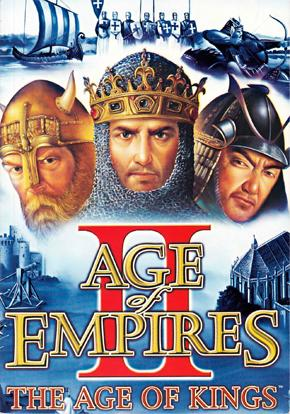
\includegraphics[width=0.3\textwidth]{imagenes/marco_teo/referentes/aoe_1.png}
\caption{Carátula del juego original.}
\label{img:aoe_1}
\end{figure}

El jugador deberá ser capaz de guiar a las unidades, gestionar las ciudades y conseguir
recursos a lo largo del escenario con el fin de derrotar a las demás facciones. Además,
se nos presenta una serie de campañas en las cuales manejaremos a grandes personajes de
la historia como `William Wallace' o `Juana de Arco' entre otros.

El juego hace de referente en varios aspectos entre los que podemos encontrar el
apartado visual donde se utiliza una perspectiva isométrica con cámara fija y el uso
de una estética clásica propia de las épocas a las que pertenecen las civilizaciones.

\begin{figure}[ht]
\centering
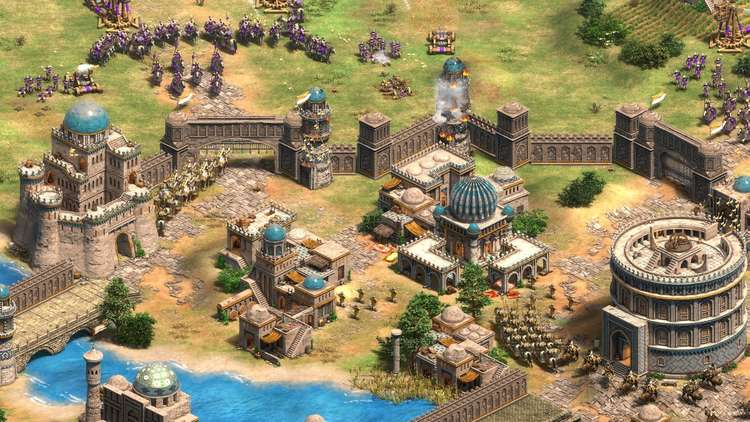
\includegraphics[width=0.7\textwidth]{imagenes/marco_teo/referentes/aoe_2.png}
\caption{Ciudad siendo asediada.}
\label{img:aoe_2}
\end{figure}

Todas la unidades de las que podemos disponer cuentan con una serie características que
las hacen más o menos fuertes en función del objetivo al que ataquen, podemos encontrar
el ejemplo de las máquinas de asedio las cuales son más fuertes contra estructuras pero
más débiles contra infanteria, o las unidades a caballo que son fuertes contra arqueros
e infanteria pero débiles frente a lanceros.
Este tipo de mécanicas dotan al juego de una importante componente táctica en el manejo
de las unidades que debemos dominar si queremos completar los diferentes niveles de
forma satisfactoria~\ref{img:aoe_2}.

\subsection{The Are Billions}
En segundo lugar podemos encontrar el juego \textit{'\acf{TaB}'} el cual reutiliza
una serie de características propias del género y como pueden ser la perspectiva
isométrica pero sin dejar de innovar introduciendo nuevas mecánicas y/o formas de
plantear la jugabilidad.

\begin{figure}[ht]
\centering

\includegraphics[width=0.7\textwidth]{imagenes/marco_teo/referentes/tab_1.png}
\caption{Imágen promocional del juego.}
\label{img:tab_1}
\end{figure}
 
En \textit{'\ac{TaB}'} podemos encontrar funciones interesantes como la pausa
táctica la cual nos permitirá visualizar detenidamente el estado del mapa sin tener que
preocuparnos por no estar atendiendo algunos posibles eventos como ataques a nuestras
tropas por parte del enemigo. En juegos anteriores como los \textit{'\ac{AoE}'} es
fácil encontrarnos en la situación de tener trabajadores en la ciudad sin hacer tareas
un rato y no poder mirar cuales son e ir pensando su ocupación siguiente por estar
atrapado en refriegas con otros jugadores, con este tipo de mecánicas estas situaciones
se solventan en mayor o menor medida y permiten al jugador tomarse el tiempo que
necesite para pensar las acciones que quiere realizar.

Otro aspecto llamativo en el podemos fijarnos es en la aparición de solamente dos
facciones. Por un lado encontramos `El Nuevo Imperio', la facción del jugador, la
cual representa una serie de colonias que tendremos que desarrollar a lo largo de
los niveles. En el otro lado encontramos las infinitas hordas de zombis que tratarán
de exterminar a la raza humana.

\begin{figure}[ht]
\centering
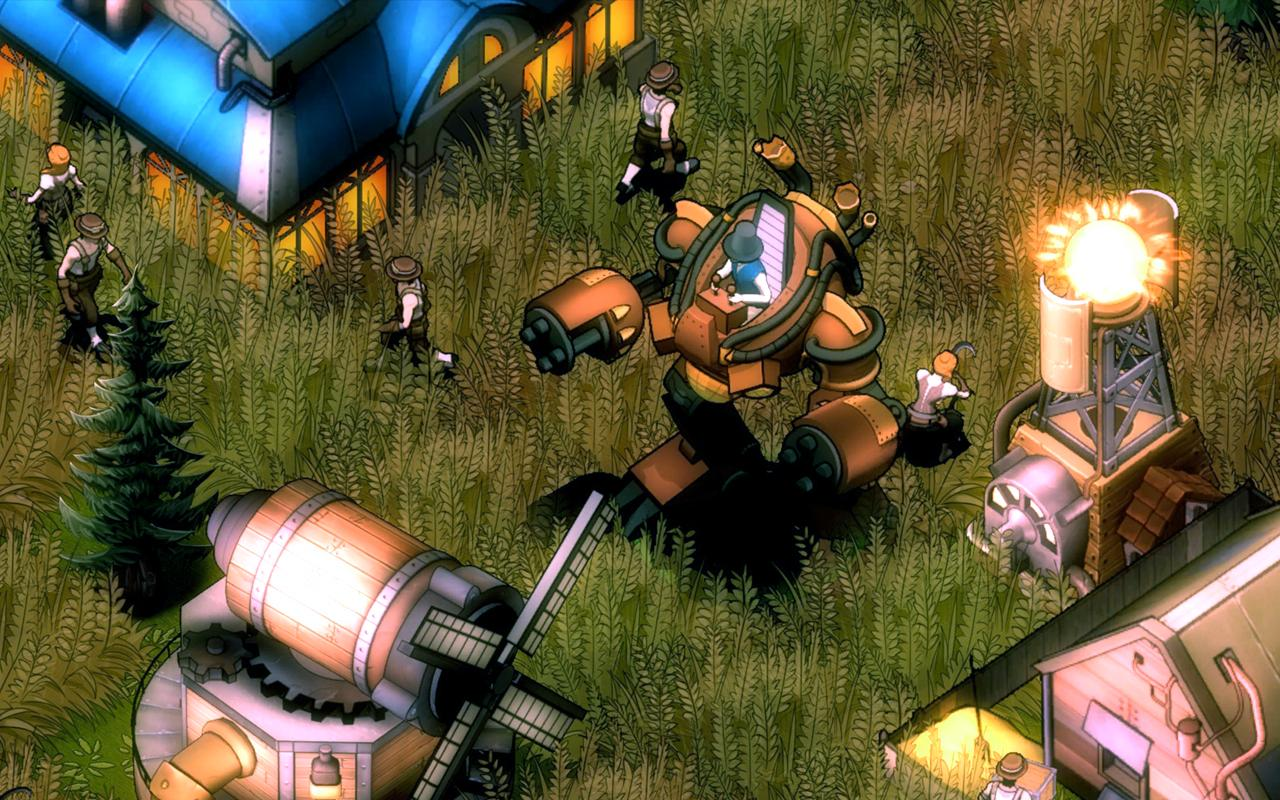
\includegraphics[width=0.6\textwidth]{imagenes/marco_teo/referentes/tab_2.png}
\caption{Ejemplo de unidad mecánica del imperio y estética del juego}
\label{img:tab_2}
\end{figure}

A diferencia de en \textit{'\ac{AoE}'} que todas la facciones poseen las mismas unidades
\footnote{Algunos valores pueden variar según bonos de facción}, en
\textit{'\ac{TaB}'} cada facción dispondrá de unidades únicas con acciones propias.
Como podemos ver en la imágen~\ref{img:tab_2} las tropas del imperio se basan en el uso
de maquinaria y armas de fuego para repeler las hordas enemigas, por otro lado los
zombis contarán con diversas caraterísticas físicas mejoradas conforme sean de mayor
``nivel'' puediendo encontrar algunos más rápidos, o más fuertes o más grandes y
resistentes al daño.~\ref{img:tab_3}

\begin{figure}[ht]
\centering

\includegraphics[width=0.5\textwidth]{imagenes/marco_teo/referentes/tab_3.png}
\caption{Infectado gigante}
\label{img:tab_3}
\end{figure}

Como último punto a destacar de la entrega tenemos la introducción del un modo de
juego de supervivencia donde a lo largo del tiempo irán apareciendo oleadas de zombis
donde cada vez aparecen más enemigos y más poderosos de forma infinita, haciendo así
que la partida termine cuando el jugador deje de aguantar la ofensiva enemiga.


\section{Técnicas de inteligencia articificial}
Como ya se ha mencionado anteriormente en la introducción~\ref{intro} de este \ac{TFG}
el grueso del desarrollo y uno de los objetivos más importantes del proyecto recaen en
el desarrollo de una \ac{IA} haciendo uso de las técnicas de \textit{'Flocking'} y
\textit{`Steering behaviors'}.

Para ello nos basaremos principalmente en las explicaciones y ejemplos que podemos
encontrar en el libro \cite[ch.~3]{Millington2009} donde de forma extensa y detallada
se nos introduce en la teoría relacionada a los algoritmos y la forma en la que estos
se estructuran e interactuan entre ellos. Para dar un poco de contexto sobre el tema
resumiremos brevemente las ideas que se nos presentan a lo largo del capitulo dedicado
a estas técnicas. 

Los \textit{`Steering behaviors'} pueden ser entendidos como una serie de algoritmos
destinados a guiar la forma en la cual los \ac{NPC} se desplazan por el escenario
y/o interactuan con los distintos elementos que puedan encontrase en la escena. Siguen
una filosofía de crear movimientos complejos a base de una combinación de movimientos 
y/o acciones simples, un ejemplo común puede ser la acción de perseguir a un objetivo
mientras se sortean obstáculos en el proceso. \\ 
En este caso no tendríamos una función llamada 
\textit{``persigue-enemigo-mientras-esquivas()''} y esta encargarse de todo el 
trabajo, sino que, tendremos el cálculo de la velocidad y dirección necesarias para
alcanzar el objetivo, la compropación para saber si hay algún tipo de
obstáculo por el camino y la rectificación de la trayectoria en caso de
haberlos cada uno por su lado y es la resultante de todos los pasos la que defina el
movimiento final.

Esta forma de estructurar y formar actividades complejas en base a acciones más simples
nos permite reutilizar y jugar con los diferentes comportamientos permitiéndonos crear
con ellos un amplio espectro de resultados.

En lo referente al \textit{'Flocking'} podemos observar como en esencia es lo mismo que
los \textit{`Steering behaviors'} pero añadiendo factores y/o componentes grupales,
el origen del modelo lo podemos encontrar en las publicaciones de \cite{Boids1986} donde
se nos introduce el concepto de \textit{``Boid''} como entidad generica que simula su
comportamiento bajo este algoritmo. Además, se nos introducen los tres comportamientos
básicos en los que se basa la técnica para generar el movimiento emergente, que son:

La \textbf{separación}~\ref{img:separation-b} que cada \textit{Boid} mantendrá entre
las demás entidades en su vencidad, con esto evitaremos solapamientos y respetar el
espacio y movimiento de las demás entidades.

\begin{figure}[ht]
\centering
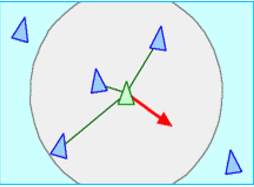
\includegraphics[width=0.35\textwidth]{imagenes/marco_teo/separation.png}
\caption{Separation behavior}
\label{img:separation-b}
\end{figure}

Por otro lado podemos encontrar el \textbf{alineamiento}~\ref{img:alignment-b} de la
dirección del movimento propio con las de las entidades más cercanas, de esta forma conseguimos un
movimiento armónico entre los \textit{boids} y produciremos una sensación de
coordinación entre ellos.

\begin{figure}[ht]
\centering
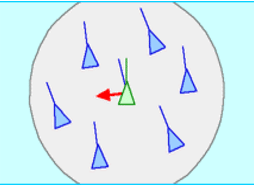
\includegraphics[width=0.35\textwidth]{imagenes/marco_teo/alignment.png}
\caption{Alignment behavior}
\label{img:alignment-b}
\end{figure}

Por último encontramos la \textbf{cohesión}~\ref{img:cohesion-b} la cual se encargará de
mantener a las entidades cercanas juntas para crear esa sensación de grupo que buscamos
con el algoritmo.

\begin{figure}[ht]
\centering
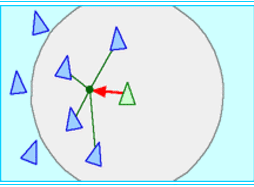
\includegraphics[width=0.35\textwidth]{imagenes/marco_teo/cohesion.png}
\caption{Cohesion behavior}
\label{img:cohesion-b}
\end{figure}

Por otro lado, podemos ver en el articulo de `Raynolds' como a lo largo de los años se
ha ido modificando y ampliando el algoritmo con el fin de añadir variaciones en el
comportamiento y/o introducir más factores influyentes en la decisión de los 
\textit{Boids} como puede ser el olor de determinada entidad/es y/o escenario. \\
Esto sin duda es gracias a la versatílidad que nos proporciona el uso de los
\textit{`Steering behaviors'} y jugar con la importancia de las distintas componentes
a la hora de hacer la toma de decisiones.


\chapter{Documento de Diseño del Juego (GDD)}
\label{GDD}

\section{Descripción general}
El juego que se pretende desarrollar se basa en el apartado de navegación por el mapa y combate
típicos en los \ac{RTS}. A lo largo de los distintos niveles, el jugador deberá hacer
frente a distintos desafíos como pueden ser: escoltar con sus unidades de un punto
del mapa a otro a un personaje importante y/o eliminar a todas las entidades enemigas del escenario.

\section{Mecánicas}
Durante el juego podremos ejecutar una serie de ordenes sobre nuestras unidades para cambiar
su distribución, ordenarles que se desplazen y/o que ataquen a enemigos.\\
Para el desplazamiento por el mapa, el jugador contará con un marcador en el mapa que podrá
mover para que sus unidades lo sigan mientras les sea posible.

\begin{figure}[ht]
\centering
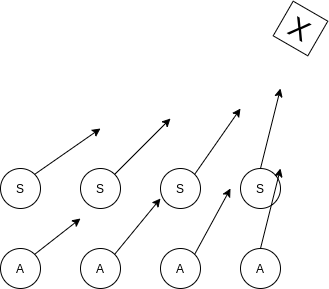
\includegraphics[width=0.35\textwidth]{imagenes/gdd/Following.png}
\caption{MockUp Seguimiento de la marca del jugador.}
\label{fig:mockup_following}
\end{figure}

En cuanto a las posibles formaciones para nuestras unidades, encontramos las siguientes:

\newpage

\begin{itemize}
\item \textbf{Sin formación:} las unidades no tendrán nigún paramétro de ordenación.

\begin{figure}[ht]
\centering
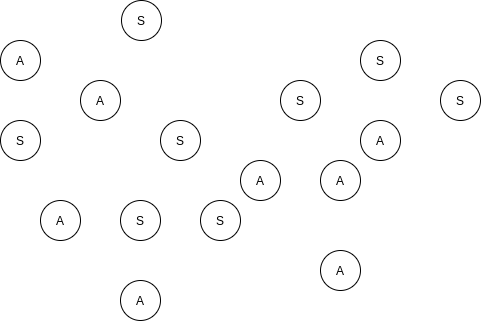
\includegraphics[width=0.32\textwidth]{imagenes/gdd/Formacion-desordenada.png}
\caption{MockUp unidades desordenada.}
\label{mockup_desordenada}
\end{figure}

\item \textbf{En anillo:} formación circular alrededor de una unidad especial. En caso de
no haber unidad escoltada el centro estará vacío. 
\end{itemize} 


\begin{figure}[ht]
\centering
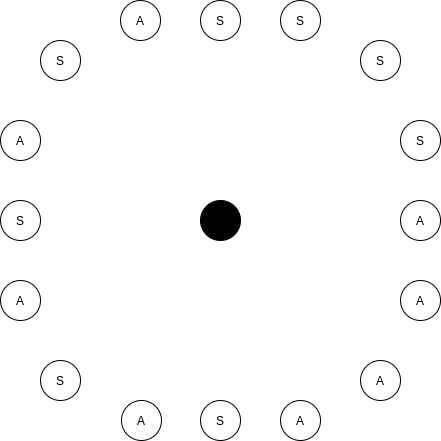
\includegraphics[width=0.32\textwidth]{imagenes/gdd/Formacion-anillo.png}
\caption{MockUp unidades en anillo.}
\label{mockup_anillo}
\end{figure}

Por último podemos ordenar a las unidades que mantengan una estrategia definida:

\begin{itemize}
\item \textbf{Huida:} en este modo las unidades seguirán el marcador sin pararse a pelear con unidades
cercanas enemigas.

\item \textbf{Agresivo:} en el momento en el que la tropa divisa un enemigo saldrá directo a atacarle,
aunque se aleje esta le seguirá mientras siga en su rango de detección.
\end{itemize} 

Aunque el jugador marque una estrategia y forma de plantear el combate, las unidades podrán
decidir si seguir al jugador o revelarse. Si los soldados cercanos están siendo masacrados
existe la posibilidad de que tengan miedo y huyan. Si las unidades enemigas nos superan en número
la unidad puede decidir si permanecer en defensa en lugar de atacar de forma activa.

\section{Unidades}
Entre las unidades podemos encontrar dos arquetipos con carácteristicas propias
que nos permitiran crear variedad en las soluciones a la hora de superar el
nivel.

Los tipos son los siguientes:
\begin{itemize}
	\item \textbf{Soldado:} es la unidad más básica que podemos encontrar en el campo de
							guerra, esta armado con una espada y posee estadísticas
							bajas.
	\item \textbf{Arquero:} va equipado con arco y flechas para atacar a distancia a
							sus rivales. Tiene menos resistencia que los soldados por
							lo que tendremos que protegerlos para asegurar su
							supervivencia.
\end{itemize}

\begin{table}[ht]
\begin{center}
\begin{tabular}{|c|c|c|c|c|}
\hline
        & Daño & Vida  & Rango  & Tiempo de ataque \\ 
\hline
\hline
Soldado & 7    & 24    & Melee & 2 seg.\\ 
\hline
Arquero & 4    & 14    & Largo & 3 seg.\\ 
\hline
\end{tabular}
\caption{Unidades y estadísticas}
\end{center}
\end{table}

\section{Controles}
A la hora de jugar tendremos una serie de teclas asignadas a las acciones que el
jugador puede realizar cuando interactúe con el juego. Para enumerarlas dividiremos las
acciones en dos grupos, dependiendo de si son para navegar por los menús o si
representan acciones durante el \textit{gameplay}.

Para avanzar por los menús usaremos la tecla \textbf{Enter} una vez estemos sobre la opción deseada o
para avanzar los mensajes explicativos del tutorial/informativos.

Las asignadas para jugar son las siguientes:
\begin{itemize}
	\item \textbf{Flechas o W/A/S/D:} mediante estas teclas podremos desplazar el puntero por el mapa.
	\item \textbf{Barra Espaciadora:} con esta otra podremos ordenar atacar a nuestras unidades,
									  si no encuentran una unidades enemiga en su rango se mantendrá
									  en seguimiento del puntero.
	\item \textbf{Ctrl:} activa el modo huída y las unidades dejarán de combatir y seguirán el
					  puntero.	
	\item \textbf{Z:} activa la formación en anillo.									  
	\item \textbf{X:} desactiva toda formación.
	\item \textbf{Ratón:} interactuar con el \textit{HUD}.
\end{itemize}

Tanto la \textbf{formación} como el \textbf{comportamiento} de las unidades se podrá cambiar desde un
pequeño \textbf{\textit{HUD}},que se encuentra en la esquina inferior izquierda.

\section{Pantallas}
Al ejecutar el programa la primera pantalla que aparecerá será la de 
inicio. Se compone del título del juego, la fecha de lanzamiento,
el nombre del desarrollador y un mensaje que nos indica que tenemos que pulsar la tecla
\textit{enter} para continuar, esta pantalla se mantendrá hasta que el jugador presione
dicha tecla.\\
Una vez pulsado el botón indicado se procederá a cargar el juego mientras se muestra
una barra que indica el progreso de cargado.

\begin{figure}[h]
\centering
\begin{minipage}[c]{0.42\linewidth}
	\hspace{9mm}
	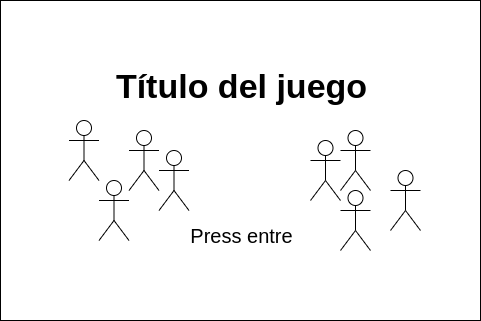
\includegraphics[width=0.7\textwidth]{imagenes/gdd/pantallas/Pantalla_ini.png}
	\caption{MockUp inicio.}
	\label{mockup_ini}
\end{minipage}
\begin{minipage}[c]{0.42\linewidth}
	\hspace{9mm}
	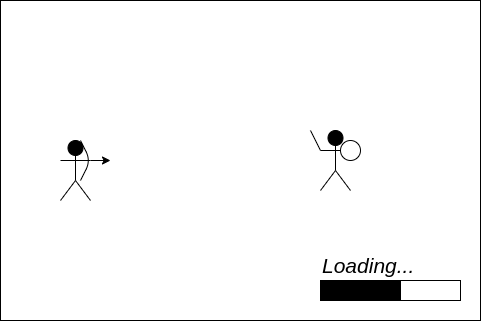
\includegraphics[width=0.7\textwidth]{imagenes/gdd/pantallas/Pantalla_carga.png}
	\caption{MockUp carga.}
	\label{mockup_carga}
\end{minipage}	
\end{figure}

A continuación de la carga nos encontraremos con el escenario, donde se desarrollará el
\textit{gameplay} y nos mantendremos en esta pantalla hasta que termine el juego, ya sea
por victoria o derrota del jugador.

\begin{figure}[ht]
\centering
\begin{minipage}[c]{0.45\linewidth}
	\hspace{9mm}
	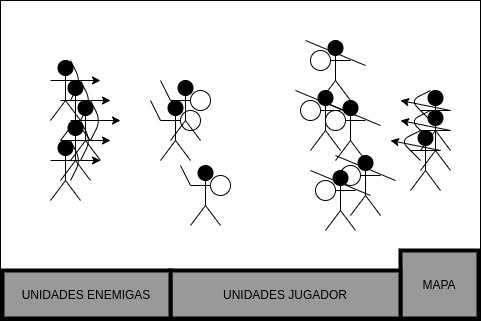
\includegraphics[width=0.7\textwidth]{imagenes/gdd/pantallas/Pantalla_gameplay.png}
	\caption{MockUp juego.}
	\label{mockup_juego}
\end{minipage}
\begin{minipage}[c]{0.45\linewidth}
	\hspace{9mm}
	
\includegraphics[width=0.7\textwidth]{imagenes/gdd/pantallas/Pantalla_pausa.png}
	\caption{MockUp pausa.}
	\label{mockup_pausa}
\end{minipage}	
\end{figure}

El final de la partida nos trae dos posibles escenarios, la victoria y la derrota. 
Para cada uno saldrá su respectivo mensaje y pasado un momento se nos mandará automáticamente a 
la pantalla de inicio.

Una última pantalla con la que el jugador podrá interactuar es la del menú de
pausa, en el cual se le dará la opción de salir o de volver a la
partida, mientras esta pantalla este activa la acción en el juego se paralizará hasta
que el jugador decida. 

\begin{figure}[ht]
\centering
\begin{minipage}[c]{0.45\linewidth}
	\hspace{9mm}
	
\includegraphics[width=0.7\textwidth]{imagenes/gdd/pantallas/Pantalla_victoria.png}
	\caption{MockUp victoria.}
	\label{mockup_victoria}
\end{minipage}
\begin{minipage}[c]{0.45\linewidth}
	\hspace{9mm}
	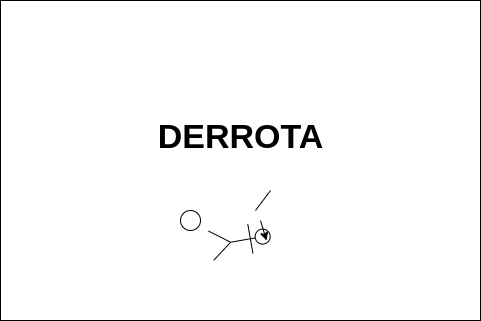
\includegraphics[width=0.7\textwidth]{imagenes/gdd/pantallas/Pantalla_derrota.png}
	\caption{MockUp derrota.}
	\label{mockup_derrota}
\end{minipage}	
\end{figure}

\section{Estados del juego}
Una vez mostradas todas las posibles pantallas con las que podrá interactuar el jugador,
es interesante dibujar un diagrama de flujo que plasme sus conexiones y posibilidades
con el fin de crear una representación gráfica que sirva como esquema global.

Dicho esquema podemos encontrarlo en la figura siguiente:

\begin{figure}[ht]
\centering
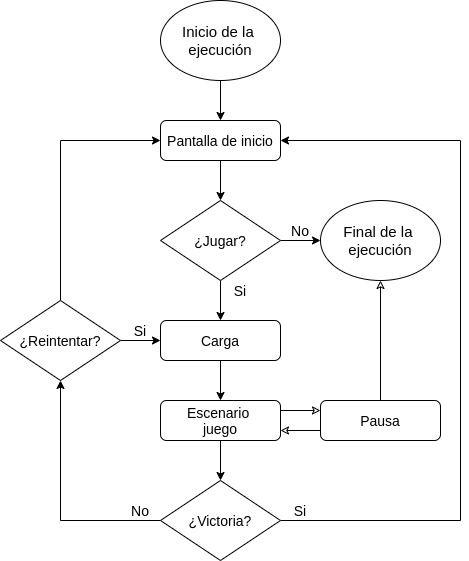
\includegraphics[width=0.45\textwidth]{imagenes/gdd/pantallas/flow_ejecucion.png}
\caption{MockUp flujo de ejecución.}
\label{esq:flow_juego}
\end{figure}

\section{Niveles}
El juego contiene actualmente 2 niveles, el primero se trata de un nivel introductorio
en el que encontraremos grupos pequeños de unidades fáciles de abatir para que el jugador conozca
cómo es el combate en el juego. Además, a lo largo del nivel pondrémos marcadores para que indiquen
al jugador cómo jugar o \textit{tips} para superar los niveles de forma satisfactoria.
El nivel se supera matando a los enemigos.

\begin{figure}[ht]
\centering
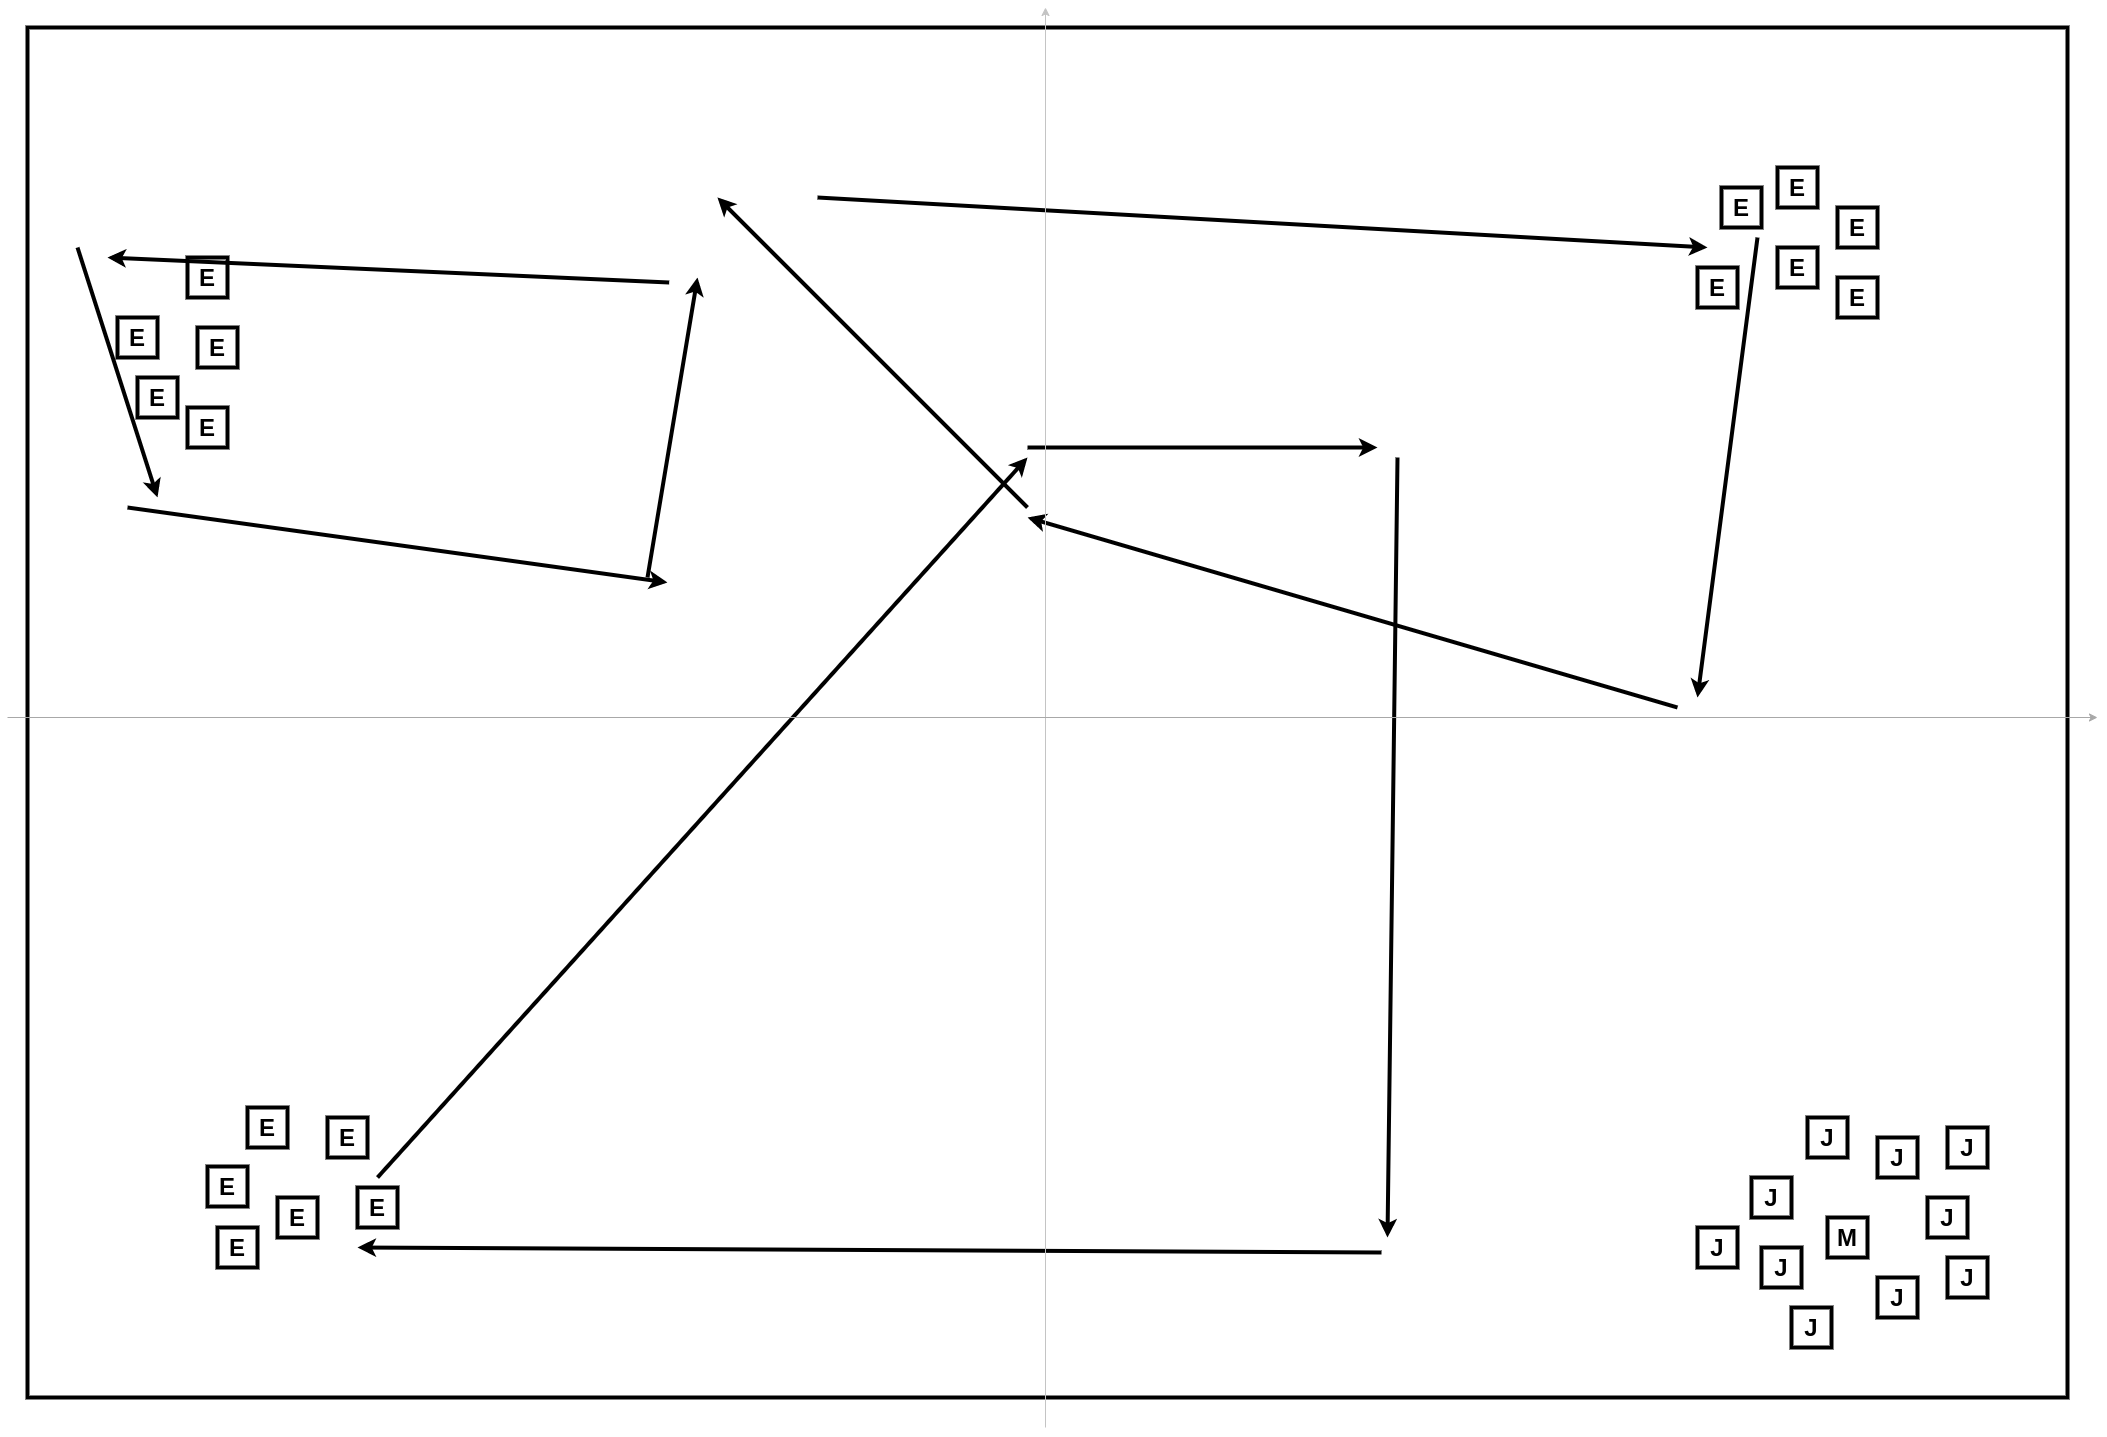
\includegraphics[width=0.6\textwidth]{imagenes/gdd/nivel0.png}
\caption{MockUp nivel 0.}
\label{esq:lvl0}
\end{figure}

En el segundo nivel se muestra otro de los objetivos posibles en el juego: alcanzar
una zona de huída/meta más allá de las tropas enemigas. En este nivel encontraremos
grupos más grandes de enemigos que nos pueden vencer y hacernos repetir el nivel, por ello podremos optar
por intentar derrotarlos o buscar una ruta que nos evite el conflicto lo máximo posible. 

\begin{figure}[ht]
\centering
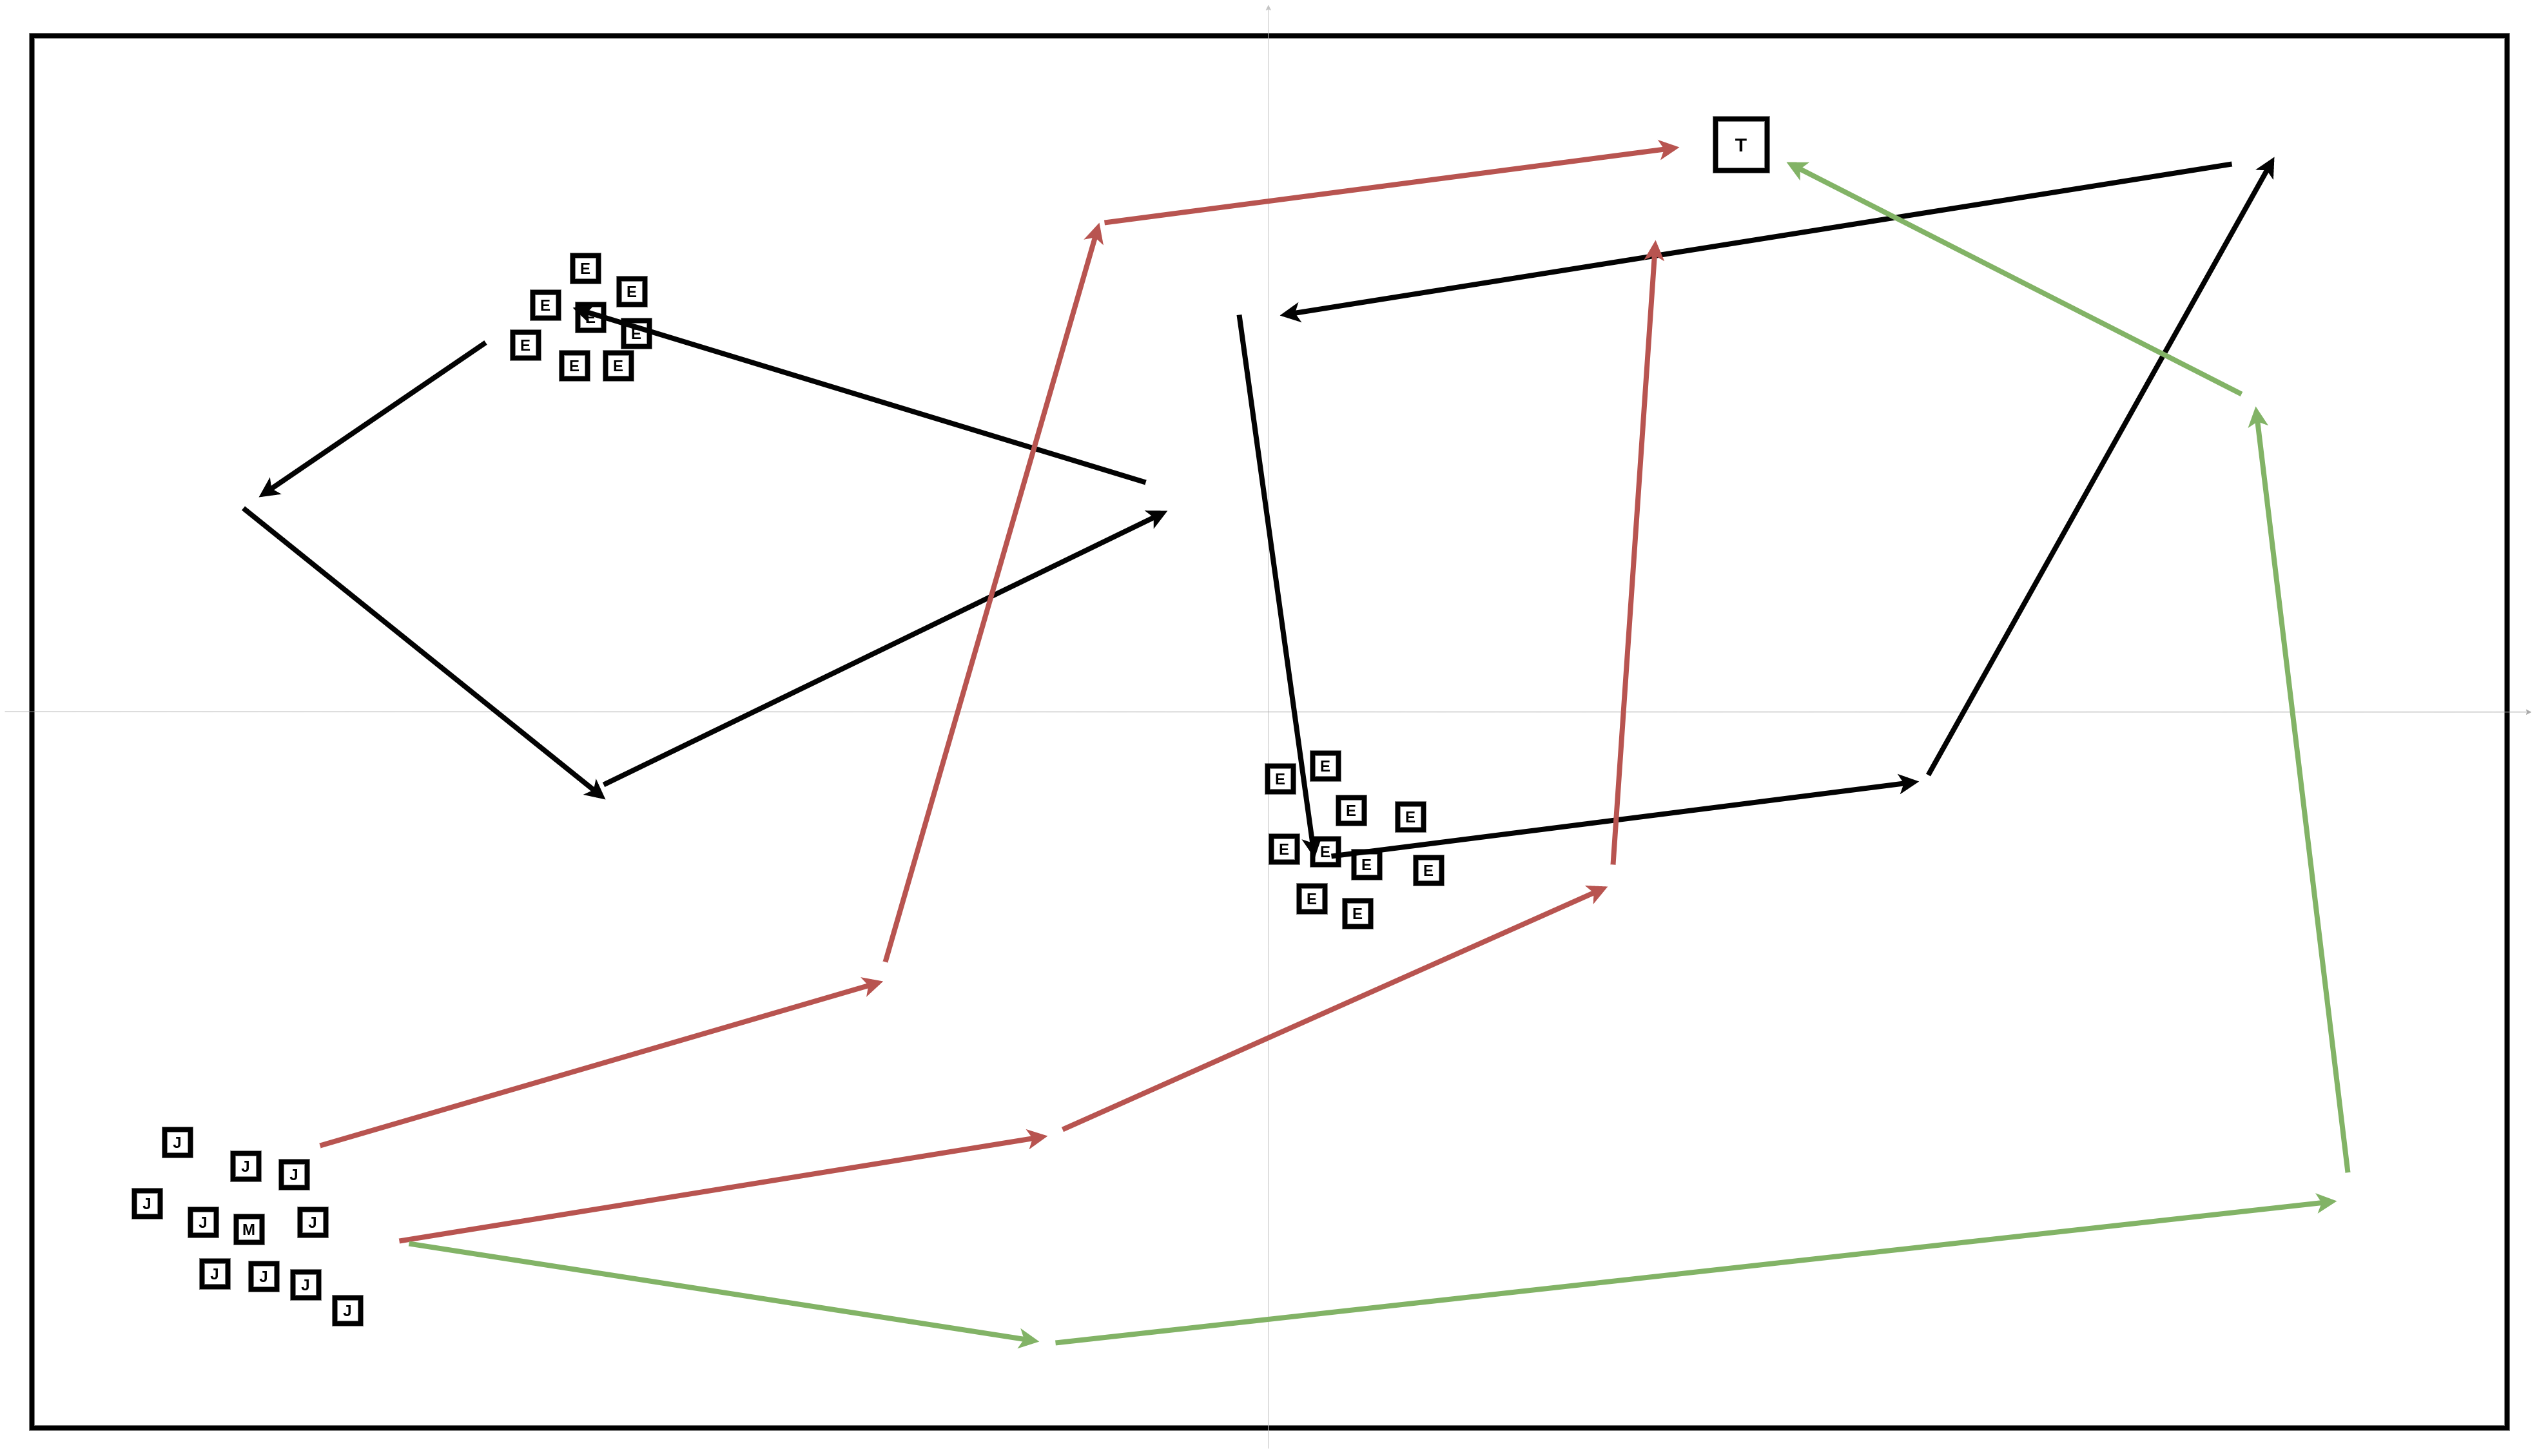
\includegraphics[width=0.6\textwidth]{imagenes/gdd/nivel1.png}
\caption{MockUp nivel 1.}
\label{esq:lvl1}
\end{figure}

\section{Escenarios}
A lo largo de los niveles la intención es que nos encontremos con distintos biomas como
pueden ser praderas, bosque o desiertos similares a los que podemos encontrar en \ac{AoE} II.

\begin{figure}[ht]
\centering
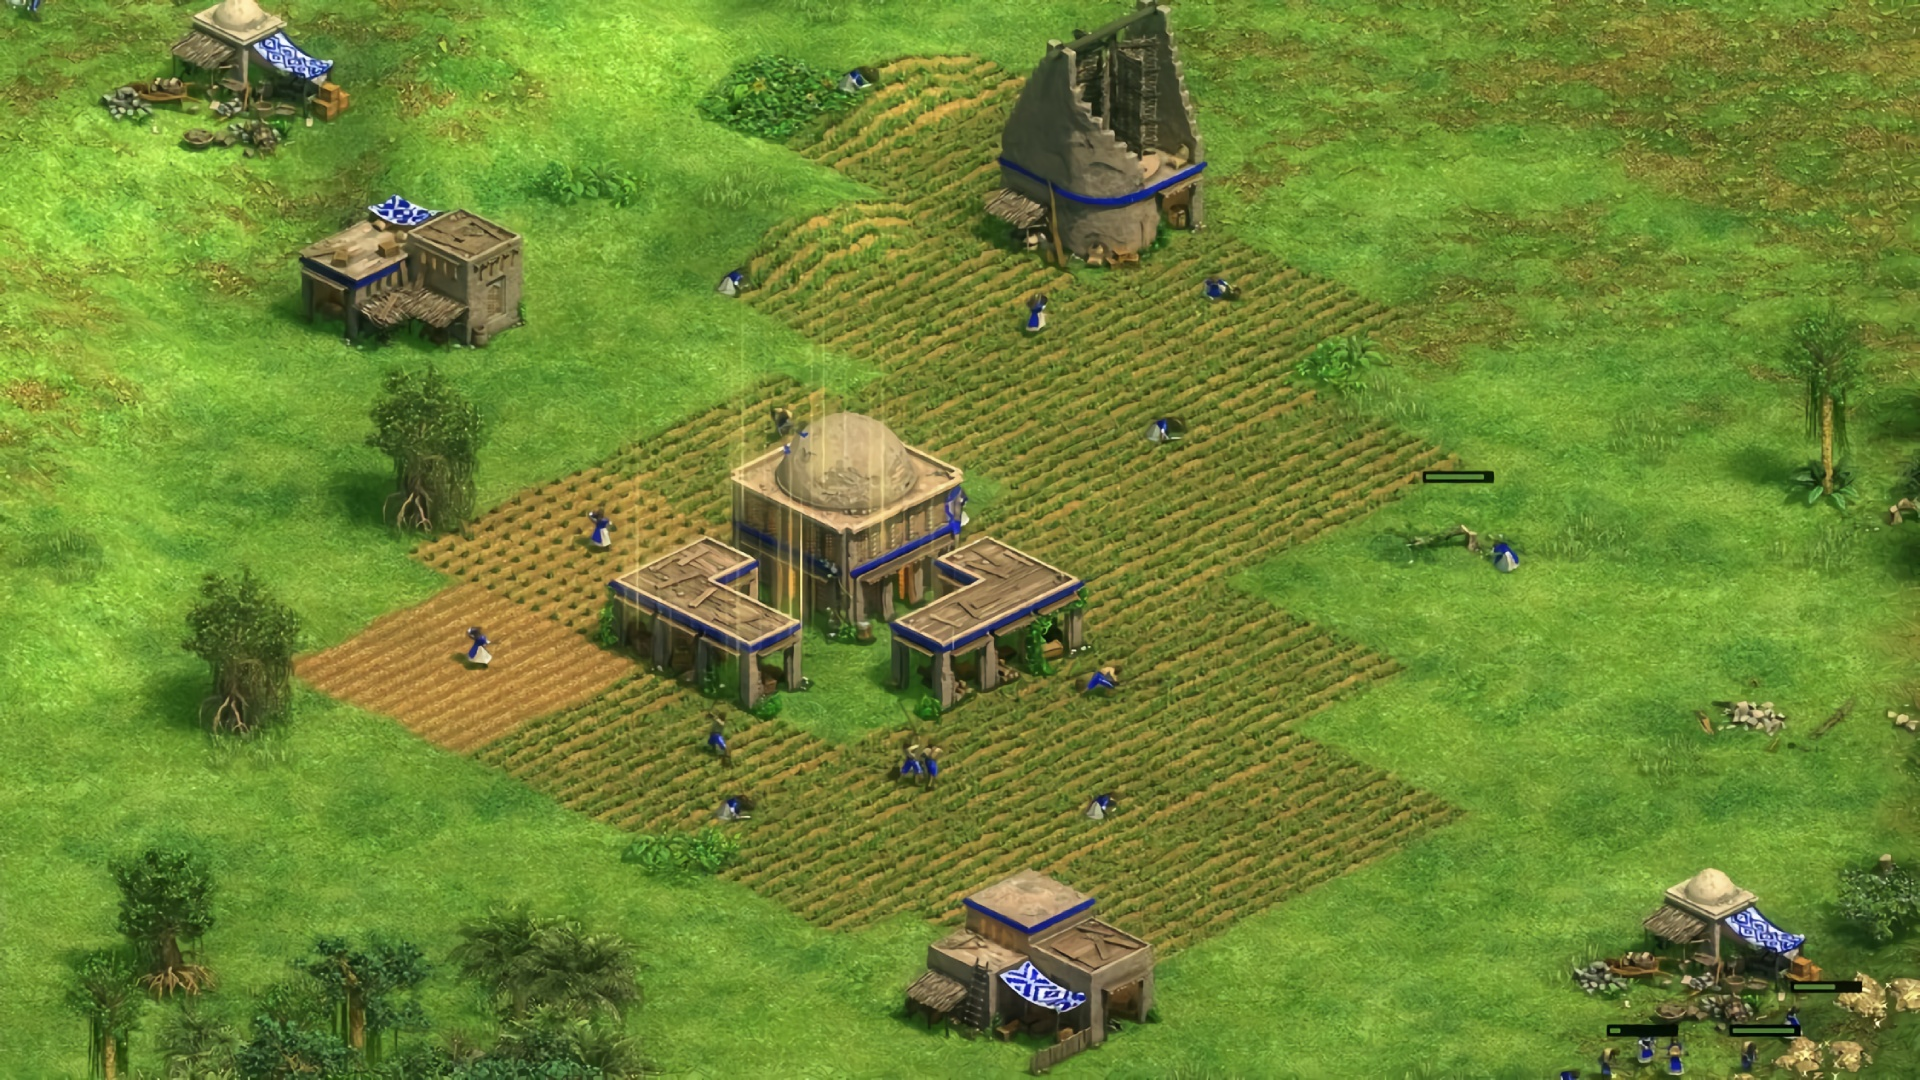
\includegraphics[width=0.6\textwidth]{imagenes/gdd/mapa_aoe_1.jpg}
\caption{Ejemplo escenario con vegetación.}
\label{img:mapa_aoe1}
\end{figure}

Además de imitar el estilo artístico el juego se desarrollará empleando una cámara
aerea fija manteniendo una perspectiva isométrica que nos permitirá visualizar desde
un punto elevado una gran porción del escenario. Esto lo haremos con el fin de dar al
jugador la posibilidad de conocer lo máximo posible el territorio cercano y a la
vez le libramos de preocuparse por situar la cámara para cada momento. \\
Al mantener una posición fija podemos situar todos los elementos en la escena de forma
que no obstaculicen la visión o molesten al jugador.

En las primeras versiones del proyecto el juego todos los elementos serán 2D y la vista será
un plano picado, el final deseable será poder pasar a un entorno 3D.

\section{Sistema de cámaras}
Si quisiéramos mostrar todo el nivel por pantalla, tendríamos el problema de que los elementos
quedarían dibujados con un tamaño demasiado pequeño si el nivel supera las dimensiones de la pantalla.
Por ello, si queremos poder diseñar niveles con las dimensiones que queramos deberemos mostrar únicamente
las fracción del nivel que ocupamos en cada momento.

En este caso, tendríamos una cámara que seguirá al puntero del jugador por el nivel y tendremos el
minimapa para poder ubicarnos en el nivel.

\section{Mínimo producto viable}
Una vez planteadas todas las características deseadas para el videojuego, es acosenjable
decidir qué partes del producto son vitales para mostrar la experiencia
de juego deseable. El hecho de marcar estos objetivos nos ayudará a poder desarrollar una
versión reducida del proyecto que nos permita dar la sensación de tener un producto acabado.\\
Es importante realizar este proceso ya que por motivos internos o externos al equipo de desarrollo,
siempre existen contratiempos que nos impidan conseguir todos los objetivos propuestos en el
documento.

En cuanto a las etapas en la ejecución del juego, encontramos esencial el poder finalizar el nivel,
ya sea por victoria o derrota. Acto seguido volver al comienzo del nivel, dejando a un lado un
posible menú inicial y de pausa.

Una vez en partida el juego constará de un nivel único compuesto por: un escenario estático
mínimo, un conjunto de unidades propiedad del jugador y otro perteneciente a la máquina.\\
Al inicio del juego el jugador se encontrará quieto en uno de los extremos del nivel y el enemigo 
estará patrullando por una zona designada, dejando así a elección del jugador la distribución y el
momento exacto en el que comenzará la disputa.

En lo referente a las mecánicas y jugabilidad, es importante que el jugador sea capaz de poder
mover a sus unidades por el escenario y ordenarles atacar. También sería deseable poder
ajustar algunos parámetros del comportamiento de su ejercito para poder pasar el nivel de más
de una forma.\\
Por otro lado, la \ac{IA} debe ser capaz de detectar el acercamiento del jugador y responder a la
ofensiva, dejando la capacidad de tomar la iniciativa y variar su estrategia para versiones
más completas. Ambos ejércitos se compondrán de soldados y arqueros.

En lo referente al apartado visual, sería deseable tener sprites para unidades y escenario pero
de ser necesario podemos mantener el sistema de \textit{render} inicial.


\section{Actualización: 13/04/21}
\begin{itemize}
	\item Corregido el movimiento lento de las entidades en algunos momentos cuando estaban en el radio
	de frenada debido a un cálculo erróneo en las diviones con el tipo de dato en coma fija.
	
	\item Creación de una componente para las colisiones e integración en los sistemas pertinentes.
	
	\item Solucionado el problema de las balas que no colisionaban bien.
	
	\item Adicción de los \textit{Colliders} al modo de depuración visual.
	
	\item Cambios ligeros en el sistema de eventos de las balas y creación y destrucción de entidades.
	
	\item Creación de un \textit{HUD} para seleccionar comportamientos y formaciones de las unidades
	aliadas.
	
	\item Rediseño completo en la toma de decisión de las unidades aliadas y enemigas.

	\item Creación de un componente de BlackBoard para el seguimiento al pj v0.1.
	
	\item Sistema de cámaras y coordenadas de mundo: ahora las dimensiones del nivel son independientes
	del tamaño de la ventana, se usan los limites del nivel para no dejar pasar a las unidades, se hace
	\textit{clipping} sobre las unidades que no están en la cámara, el minimapa ahora muestra la porción
	de nivel que se muestra.
	
	\item Se ha mejorado el sistema de entidades objetivo y los mensajes de muerte y ataque para cambiar
	de objetivo cuando el actual muera, además al morir una unidad se eliminan los demás mensajes asociados
	a ella.

	\item El componente de \ac{IA} ya no contiene la ruta directamente, ahora contiene un iterador a su
	ruta y se ha creado el tipo de dato ruta con operadores sobrecargados para navegar por ella. También
	tenemos ``caminos'' diseñados pero sin incluir, los cuales son caminos no cíclicos.

	\item Se ha ampliado un poco el GDD con apartados sobre tareas pendientes y objetivos.

	\item En el diario de desarrollo se han sustituido códigos de ejemplo por mockups.  
\end{itemize}

\section{Actualización: 06/05/21}
\begin{itemize}
	\item Redacción problema en las divisiones de los enteros con coma fija.

	\item Redacción problema con las colisiones y solución.

	\item Redacción \textit{HUD} v0.4.
	
	\item Redacción sistema de cámaras en el GDD y diario de desarrollo.

	\item Redacción cambios en las entidades: rutas y comportamientos.
\end{itemize}

%input{capitulos/objetivos}
%input{capitulos/metodologia}
%input{capitulos/desarrollo}
%input{capitulos/resultados}
%input{capitulos/conclusiones}

%\nocite{*} %incluye TODOS los documentos de la base de datos bibliográfica sean o no citados en el texto
\nocite{*}
\bibliography{bibliografia/bibliografia.bib}\addcontentsline{toc}{chapter}{Bibliografía} %sustituir bibliografía con el nombre del fichero bibtex con la bibliografía
\bibliographystyle{apalike}
%
%\appendix
%\chapter{Anexo I}
Aquí vendría en anexo I 

\end{document}
